\documentclass[a4paper,10pt]{article}

\usepackage[french]{babel}
\usepackage[T1]{fontenc}
\usepackage[utf8]{inputenc}
\usepackage{amsmath}
\usepackage{graphicx}
\usepackage[colorinlistoftodos,prependcaption,textsize=tiny]{todonotes}
\usepackage{eurosym}
\usepackage{appendix}%[toc,page]
\usepackage{varioref}
\usepackage{float}
\usepackage[numbered,bw]{mcode}
\usepackage{listing}

%3 lignes suivantes : Remet le compteur de section à 0 à chaque nouvelle partie
\makeatletter
\@addtoreset{section}{part}
\makeatother

%Change l'apparence des itemize
\renewcommand{\labelitemi}{\textbullet}

\title{Analyse décisionnelle pour l'entreprise FaBrique}
\author{Heptanôme 4203}
\date{\today}

\begin{document}
\maketitle 

%%%%%%%%%%%%%%%%%%%%%%%%%%%%%%%%
%%%%%%%% Introduction %%%%%%%%%%
%%%%%%%%%%%%%%%%%%%%%%%%%%%%%%%%

\section*{Membres du groupe}
\begin{itemize}
\item Nicolas \textsc{Bonfante}
\item Cédric \textsc{Boscher}
\item Romain \textsc{Bourrier}
\item Marion \textsc{Chalumeau}
\item Charles \textsc{de Lacombe}
\item Ophélie \textsc{Delsaux}
\item Nicolas \textsc{Nadisic}
\end{itemize}

\section*{Introduction}

  L'entreprise FaBrique a émis une demande d'analyse décisionnelle concernant la mise en place d'un plan de fabrication hebdomadaire optimal. L'entreprise fabrique différentes gammes de produits grâce à l'utilisation de machines au sein de sa structure. La demande du client nous impose de respecter des contraintes logistiques au sein de l'entreprise, mais également d'analyser les besoins unitaires de chaque responsable. Dans un premier temps, nous chercherons une solution optimale répondant de manière individuelle aux besoins de chaque responsable, tout en tenant compte des contraintes identifiées au préalable. Avec la consultation du responsable d'entreprise et de manière à fournir un unique plan optimal pour toute l'entreprise, nous réaliserons une analyse multicritère afin d'établir un plan permettant un compromis satisfaisant pour chacune des parties. Nous inclurons systématiquement l'analyse et la modélisation mathématique effectuées en amont de la résolution du problème.
  
\newpage
\tableofcontents

%%%%%%%%%%%%%%%%%%%%%%%%%%%%%%%%%%%%%%%%
%%%%%% Partie PROG MONOCRITERE %%%%%%%%
%%%%%%%%%%%%%%%%%%%%%%%%%%%%%%%%%%%%%%%%
\newpage
\part{Modélisation des contraintes et des objectifs}
\begin{large}
\emph{Programmation linéaire monocritère}
\end{large}

%%%%%%%%%%%%%%%%%%%%%%%%%%%%%%%%%%%%%%%%%%%%
%%%%%% Modélisation des contraintes %%%%%%%%
%%%%%%%%%%%%%%%%%%%%%%%%%%%%%%%%%%%%%%%%%%%%

\section{Modélisation des contraintes}
L'analyse des contraintes est un facteur clé dans la réalisation d'un nouveau plan de développement pour l'entreprise ainsi que la première étape de notre étude.
\vspace{\baselineskip}

Conformément aux besoins clients émis, nous veillerons dans un premier temps à prendre en compte \textbf{la fabrication d'au moins 5 unités de produit A et 5 unités de produit B par semaine}. Afin d'établir un modèle mathématique cohérent, \textbf{nous veillerons également à éliminer les cas où la quantité de produits C, D, E ou F serait négative}.\newline

Notons $n_X$ le nombre de produits de dénomination X à produire par l'intermédiaire du plan de fabrication. Lors de l'exécution du plan, nous veillerons donc à respecter les critères suivants :

$$n_A \geq 5$$
$$n_B \geq 5$$
$$n_C \geq 0$$
$$n_D \geq 0$$
$$n_E \geq 0$$
$$n_F \geq 0$$

Nous établirons de plus un plan de fabrication \textbf{respectant les contraintes de stockage des matières premières dans l'entreprise}.

De manière à respecter ces critères, nous ne dépasserons pas l'utilisation de :
\newline
\begin{itemize}
\item 350 unités de matière 1
\item 620 unités de matière 2
\item 485 unités de matière 3\newline
\end{itemize}

Compte-tenu des quantités de matières premières nécessaires à la fabrication de chaque objet, nous modélisons cette contrainte de la manière suivante :
\newline
\begin{itemize}
\item[\textbullet]  \textbf{Matière 1 :} $n_A + 2 \times n_B + n_C + 5 \times n_D + 2 \times n_F \leq 350$
\item[\textbullet]  \textbf{Matière 2 :} $2 \times n_A + 2 \times n_B + n_C + 2 \times n_D + 2 \times n_E + n_F \leq 620$
\item[\textbullet]  \textbf{Matière 3 :} $n_A + 3 \times n_C + 2 \times n_D + 2 \times n_E \leq 485$\newline
\end{itemize}

Pour finir, nous veillerons à ne pas sur-solliciter les machines dans le cadre du plan de fabrication établi, de manière à ce qu'il puisse être exécuté dans un mode de fonctionnement des machines en 2 huit, 5 jours sur 7, soit 4800 minutes par semaine. Compte-tenu des temps unitaires d'usinage de chaque produit sur chaque machine, nous fournissons le modèle suivant :
\newline
\begin{itemize}
\item[\textbullet] \textbf{Machine 1 :} $8 \times n_A + 15 \times n_B + 5 \times n_D + 10 \times n_F \leq 4800$
\item[\textbullet] \textbf{Machine 2 :} $7 \times n_A + 12 \times n_B +2 \times n_C + 15 \times n_D + 7 \times n_E + 12 \times n_F \leq 4800$
\item[\textbullet] \textbf{Machine 3 :} $8 \times n_A + n_B + 11 \times n_C + 10 \times n_E + 25 \times n_F \leq 4800$
\item[\textbullet] \textbf{Machine 4 :} $2 \times n_A + 10 \times n_B + 5 \times n_C + 4 \times n_D + 13 \times n_E + 7 \times n_F \leq 4800$
\item[\textbullet] \textbf{Machine 5 :} $5 \times n_A + 8 \times n_C + 7 \times n_D + 10 \times n_E + 25 \times n_F \leq 4800$
\item[\textbullet] \textbf{Machine 6 :} $5 \times n_A + 5 \times n_B + 3 \times n_C + 12 \times n_D + 8 \times n_E + 6 \times n_F \leq 4800$
\item[\textbullet] \textbf{Machine 7 :} $5 \times n_A + 3 \times n_B +5 \times n_C +8 \times n_D + 7 \times n_F \leq 4800 $\newline
\end{itemize}


\fbox{
\begin{minipage}{1\textwidth}
     \begin{center}
     
     \textbf{\textit{Modèle récapitulatif des contraintes}}
			$$n_A \geq 5$$ 
			$$n_B \geq 5$$ 
			$$n_C \geq 0$$ 
			$$n_D \geq 0$$
			$$n_E \geq 0$$ 
			$$n_F \geq 0$$ 
			$$n_A + 2 \times n_B + n_C + 5 \times n_D + 2 \times n_F \leq 350$$
			$$2 \times n_A + 2 \times n_B + n_C + 2 \times n_D + 2 \times n_E + n_F \leq 620$$
			$$n_A + 3 \times n_C + 2 \times n_D + 2 \times n_E \leq 485$$
			$$8 \times n_A + 15 \times n_B + 5 \times n_D + 10 \times n_F \leq 4800$$
			$$7 \times n_A + 12 \times n_B +2 \times n_C + 15 \times n_D + 7 \times n_E + 12 \times n_F \leq 4800$$
			$$8 \times n_A + n_B + 11 \times n_C + 10 \times n_E + 25 \times n_F \leq 4800$$
			$$2 \times n_A + 10 \times n_B + 5 \times n_C + 4 \times n_D + 13 \times n_E + 7 \times n_F \leq 4800$$
			$$5 \times n_A + 8 \times n_C + 7 \times n_D + 10 \times n_E + 25 \times n_F \leq 4800$$
			$$5 \times n_A + 5 \times n_B + 3 \times n_C + 12 \times n_D + 8 \times n_E + 6 \times n_F \leq 4800$$
			$$5 \times n_A + 3 \times n_B +5 \times n_C +8 \times n_D + 7 \times n_F \leq 4800 $$
               
     \end{center}
\end{minipage}
}
\vspace{\baselineskip}

Après avoir analysé les contraintes relatives au fonctionnement logistique de l'entreprise, nous effectuons \textbf{une analyse des besoins émis par chacun des responsables} au sein de la structure.

%%%%%%%%%%%%%%%%%%%%%%%%%%%%%%%%%%%%%%%%%%
%%%%%% Modélisation des objectifs %%%%%%%%
%%%%%%%%%%%%%%%%%%%%%%%%%%%%%%%%%%%%%%%%%%

\section{Modélisation des objectifs}

%%%%%%%%%%%%%%%%%%%%%%%%%%%%%%%%%%%%%%%%%%%%
%%%%%%%%%%%%%%%% Comptable %%%%%%%%%%%%%%%%%
%%%%%%%%%%%%%%%%%%%%%%%%%%%%%%%%%%%%%%%%%%%%

\subsection{Comptable}

\emph{NB : Les calculs plus détaillés de cette section sont disponibles en annexe, page \pageref{annexe}.} \\

L'objectif principal du comptable est de réaliser le plus grand bénéfice possible, ceci en tenant compte non seulement des coûts de fonctionnement des machines mais également du coût d'achat des matières premières. De cette façon, nous déduisons la fonction $G_1$ à maximiser:

$$G_1(N) = 5,833 \times n_A + 11,617 \times n_B + 12,17 \times n_C + 1,3 \times n_D + 31,65 \times n_E + 27,48 \times n_F$$

Les coefficients devant chaque $n_X$, c'est-à-dire les bénéfices à la vente du produit X, ont été calculés compte tenu du coût des matières premières, du coût d'utilisation des machines et des bénéfices à la vente de chaque produit fini.\newline


La fonction $G$ à minimiser est donc :

$$G(N) = -5,833 \times n_A - 11,617 \times n_B - 12,17 \times n_C - 1,3 \times n_D - 31,65 \times n_E - 27,48 \times n_F$$

La solution de base trouvée en utilisant les contraintes de l'entreprise est la fabrication minimale de :\newline
\begin{itemize}
\item[\textbullet] 5 produits A
\item[\textbullet] 18,16 produits B
\item[\textbullet] 0 produit C
\item[\textbullet] 0 produit D
\item[\textbullet] 240 produits E
\item[\textbullet] 93,67 produits F\newline
\end{itemize}
Le bénéfice s'échelonne ainsi à environ + 10 410,62 unités.\newline

Cette solution semble cohérente et réaliste car les produits qui doivent être le plus produits sont les produits possédant la plus grande valeur ajoutée. Remarquons le bénéfice moyen d'environ 30 unités, très proche du bénéfice maximum fait sur un produit (le produit E) qui est de 31 unités.

%%%%%%%%%%%%%%%%%%%%%%%%%%%%%%%%%%%%%%%%%%%%
%%%%%%%%%% Responsable d'atelier %%%%%%%%%%%
%%%%%%%%%%%%%%%%%%%%%%%%%%%%%%%%%%%%%%%%%%%%

\subsection{Responsable d'atelier}

L'objectif du responsable d'atelier consiste à fabriquer une quantité maximale de produits. Cela se traduit par la fonction $F_1$ à maximiser :

$$F_1(N) = n_A + n_B + n_C + n_D + n_E + n_F$$

d'où $F$ à minimiser suivante :
$$F(N) = - n_A - n_B - n_C - n_D - n_E - n_F$$

La solution de base trouvée en utilisant les contraintes de l'entreprise est la fabrication minimale de :\newline
\begin{itemize}
\item[\textbullet] 5 produits A
\item[\textbullet] 54,64 produits B
\item[\textbullet] 38,86 produit C
\item[\textbullet] 0 produit D
\item[\textbullet] 181,72 produits E
\item[\textbullet] 98,43 produits F\newline
\end{itemize}
Le nombre de produits réalisés serait donc de 378,64 produits au total, toutes gammes confondues.

%%%%%%%%%%%%%%%%%%%%%%%%%%%%%%%%%%%%%%%%%%%%
%%%%%%%%% Responsable des stocks %%%%%%%%%%%
%%%%%%%%%%%%%%%%%%%%%%%%%%%%%%%%%%%%%%%%%%%%

\subsection{Responsable des stocks}

Le but du responsable des stocks est de minimiser le nombre de produits et la quantité de matière première dans son stock. Cependant, en considérant cet objectif isolé, nous en arrivons de manière évidente à la conclusion que fermer l'entreprise serait l'option la plus adaptée. C'est pourquoi nous ajoutons une contrainte de réalisme, modélisant le fait que l'entreprise reste en activité.\newline

Nous avons calculé (lors des calculs pour le responsable d'atelier, pour maximiser la production) que la production maximale hebdomadaire de l'entreprise était de 378,64 produits. Afin de tendre vers un modèle cohérent, nous avons décidé que la production minimale pour que l'entreprise garde son activité, serait de 80\% de la production maximale, soit 300 produits par semaine.\newline

%%%%%%% LE CROUPIONG%%%%%%%%%%

Le "coût de stockage" d'un produit est égal à la quantité de matières premières utilisées pour la fabrication de ce produit, à laquelle on ajoute 1 (pour le produit lui-même). Nous obtenons donc la fonction $H$ à minimiser suivante :
$$ H(N)=  5n_A + 5n_B + 6n_C +10n_D + 5n_E + 4n_F $$

Pour satisfaire cet objectif, tout en respectant les contraintes de départ, nous devons suivre le plan de production hebdomadaire suivant :\newline
\begin{itemize}
\item[\textbullet] 5 produits A
\item[\textbullet] 32,40 produits B
\item[\textbullet] 0 produits C
\item[\textbullet] 0 produits D
\item[\textbullet] 122,5 produits E
\item[\textbullet] 140,1 produits F\newline
\end{itemize}

On arrive à un stockage optimal de 1359,9 unités.

Ce résultat est parfaitement cohérent car les produits E et F sont ceux qui nécessitent le moins de matières premières et donc qui occupent le moins de stock. Le produit F est le plus adapté mais il est plus long à produire et une production avec plus de produits F ne respecterait pas la contrainte de production minimale hebdomadaire.

%%%%%%%%%%%%%%%%%%%%%%%%%%%%%%%%%%%%%%%%%%%%
%%%%%%%%% Responsable commercial %%%%%%%%%%%
%%%%%%%%%%%%%%%%%%%%%%%%%%%%%%%%%%%%%%%%%%%%

\subsection{Responsable commercial}

Le but du responsable commercial est d'équilibrer les quantités de produits A et E. Avec ce seul objectif, il existe une infinité de solutions possibles, nous devons donc ajouter une contrainte.

Nous considérons une contrainte d'égalité entre les quantités de produits A et E, avec l'objectif de produire le plus de produits possibles. Nous allons donc, comme lors de l'étude des objectifs du responsable de l'atelier, minimiser la fonction :
$$F(N) = - n_A - n_B - n_C - n_D - n_E - n_F$$.
Cette fois, nous ajoutons une contrainte supplémentaire :
$$n_A = n_E$$
Nous obtenons le plan de production hebdomadaire suivant :
\begin{itemize}
\item[\textbullet] 119,08 produits A
\item[\textbullet] 6,92 produits B
\item[\textbullet] 42,58 produits C
\item[\textbullet] 0 produits D
\item[\textbullet] 119,08 produits E
\item[\textbullet] 87,25 produits F\newline
\end{itemize}

Nous avons ainsi bien autant de produits A que de E à la fin de la semaine, tout en conservant une production de 374,92 produits, soit 99\% du nombre de produits maximum produits sur une semaine.


%%%%%%%%%%%%%%%%%%%%%%%%%%%%%%%%%%%%%%%%%%%%%%
%%%%%%%%% Responsable du personnel %%%%%%%%%%%
%%%%%%%%%%%%%%%%%%%%%%%%%%%%%%%%%%%%%%%%%%%%%%

\subsection{Responsable du personnel}

L'objectif principal du responsable du personnel est de \textbf{limiter l'utilisation de la machine 4}, qui est très délicate. De cette façon, nous en déduisons la fonction $J$ à minimiser suivante :

$$J(N)=2 \times n_A + 10 \times n_B + 5 \times n_C + 4 \times n_D + 13 \times n_E + 7 \times n_F$$

Cette fonction correspond à la modélisation de l'utilisation de la machine 4. Il s'agit ici de minimiser la somme des temps pour produire les différentes pièces. Nous utilisons, pour résoudre ce problème, les contraintes exposées dans la première partie de l'analyse.\\

La 1\iere{} solution de base trouvée en utilisant les contraintes de l'entreprise est la fabrication de :\newline
\begin{itemize}
\item[\textbullet] 5 produits A
\item[\textbullet] 5 produits B
\item[\textbullet] 0 produits C
\item[\textbullet] 0 produits D
\item[\textbullet] 0 produits E
\item[\textbullet] 0 produits F\newline
\end{itemize}
Ce qui correspond à une utilisation de 60 minutes de la machine 4.\newline

Cette solution est logique car tout les produits utilisent la machine 4 donc plus la production est faible, moins cette machine est utilisée.\\

Cette solution n'étant pas réaliste, nous avons décidé d'intégrer une contrainte supplémentaire sur le nombre de produits à fabriquer. Nous souhaitons que la somme des produits fabriqués soit supérieure à 300 pièces à réaliser, soit environ 80\% de la production maximale de pièces.
Ceci se modélise par l'ajout de la contrainte suivante :\\

$$n_A + n_B + n_C + n_D + n_E + n_F \geq 300$$
d'où $$-n_A -n_B -n_C -n_D -n_E -n_F \leq -300$$

Nous obtenons donc un total de :\newline
\begin{itemize}
\item[\textbullet] 295 produits A
\item[\textbullet] 5 produits B
\item[\textbullet] 0 produits C
\item[\textbullet] 0 produits D
\item[\textbullet] 0 produits E
\item[\textbullet] 0 produits F\newline
\end{itemize}
Cela correspond à une utilisation de 640 minutes de la machine 4.\newline

Cette solution est logique car le produit nécessitant le moins la machine est le produit A (2 minutes). Elle semble également plus réaliste car elle respecte au mieux la demande du responsable personnel.



%%%%%%%%%%%%%%%%%%%%%%%%%%%%%%%%%%%%%%%%
%%%%%% Partie PROG MULTICRITERE %%%%%%%%
%%%%%%%%%%%%%%%%%%%%%%%%%%%%%%%%%%%%%%%%
\newpage
\part{Programmation linéaire multicritère}

Dans cette partie, nous considérons le point de vue du responsable d'entreprise. On veut construire une solution multicritère satisfaisant au mieux l'ensemble des objectifs de chaque responsable. Pour cela, nous allons déterminer le \emph{point de mire} et la \emph{matrice des gains}. Nous nous ramènerons à un problème de programmation linéaire afin de construire une \textbf{solution de compromis}.

\section{Détermination du point de mire}
Nous cherchons le point de mire, c'est-à-dire la situation idéale, mais non réaliste, où tous les critères seraient parfaitement satisfaits.

Nous prenons donc les extremas de chaque critère : maximum si le critère est à maximiser, minimum dans le cas inverse.
Les extremas ont été calculés en partie 1 et sont rappelés ici :
\label{optimum}
\begin{itemize}
\item Comptable : Bénéfice de 10410,62 unités maximum
\item Atelier : Production de 378,64 produits maximum
\item Stocks : Stock de 1359,9 unités minimum
\item Personnel : Temps d'utilisation de la machine 4 de 640 minutes minimum
\end{itemize}

L'objectif du responsable commercial n'apparaît pas. En effet, nous avons considéré, en accord avec le client, que son critère était de maximiser la production et que l'équilibre des produits A et E devenait une contrainte. Ainsi, son critère était redondant avec celui du comptable.

Maintenant que le point de mire est défini, nous allons chercher une solution optimale, qui soit incluse dans les domaines de chaque critère et qui s'approche au maximum du point de mire.

\section{Matrice des gains}

Afin de modéliser le problème, il est nécessaire de réaliser la matrice des gains  correspondant à l'ensemble des objectifs.
%% LE CROUPIONG : LA RESURRECTION DU RETOUR DE LA VENGEANCE%%
Il s'agit ici de déterminer comment chaque solution unitaire, optimale pour un objectif, répond aux autres objectifs.

Vous pouvez voir le tableau représentant la matrice à la page \pageref{tab:matgain}.

\begin{table}[H]
\centering
\caption{Matrice des gains}
\label{tab:matgain}
\begin{tabular}{c|p{0.15\linewidth}|p{0.15\linewidth}|p{0.15\linewidth}|p{0.15\linewidth}|p{0.15\linewidth}|}
\cline{2-5}
 & \multicolumn{1}{p{0.15\linewidth}|}{\textbf{Quantité Produits F(X)}} & \multicolumn{1}{c|}{\textbf{Bénéfice G(X)}} & \multicolumn{1}{p{0.15\linewidth}|}{\textbf{Quantité Stockage H(X)}} & \multicolumn{1}{p{0.15\linewidth}|}{\textbf{Temps Machine 4 J(X)}} & \multicolumn{1}{p{0.15\linewidth}|}{\textbf{Différence de qtté A/E K(X)}} \\ \hline
\multicolumn{1}{|p{0.15\linewidth}|}{\textbf{Quantité Produits Optimale}} & 378,64 & 9592,99 & 1833,64 & 3802,01 & 176,72 \\ \hline
\multicolumn{1}{|p{0.15\linewidth}|}{\textbf{Bénéfice Optimal}} & 356,84 & 10410,31 & 1690,51 & 3967,35 & 255\\ \hline
\multicolumn{1}{|p{0.15\linewidth}|}{\textbf{Quantité Stockage Optimal}} & 300 & 8132,69 & 1359,90 & 2907,19 & 117,50\\ \hline
\multicolumn{1}{|p{0.15\linewidth}|}{\textbf{Temps Machine 4 Optimal}} & 300 & 1778,82 & 1500 & 640 & 295\\ \hline
\multicolumn{1}{|p{0.15\linewidth}|}{\textbf{Différence A/E Optimale}} & 374,92 & 7459,74 & 1829,92 & 2679,08 & 0\\ \hline

\end{tabular}
\end{table}


\section{Recherche de la solution de compromis}

Pour déterminer une solution de compromis, nous allons nous ramener à un problème monocritère. L'objectif le plus important sera considéré comme notre critère, et les autres seront considérés comme des contraintes. Tant qu'un compromis n'est pas trouvé, nous dégraderons progressivement certaines contraintes.

Nous avons décidé que l'objectif prépondérant était celui du comptable : maximiser les bénéfices. La formule correspondante est donc :
$$G_1(N) = 5,833 \times n_A + 11,617 \times n_B + 12,17 \times n_C + 1,3 \times n_D + 31,65 \times n_E + 27,48 \times n_F$$

On cherche à maximiser cette fonction.

Les autres critères sont considérés comme des contraintes et représentés par les formules suivantes :
$$ - n_A - n_B - n_C - n_D - n_E - n_F < x_1 $$
$$ 5n_A + 5n_B + 6n_C + 10n_D + 5n_E + 4n_F < x_2 $$
$$ 2n_A + 10n_B + 5n_C + 4n_D + 13n_E + 7n_F < x_3 $$
$$ - n_A - n_B - n_C - n_D - n_E - n_F < x_4 $$ 

On constate que la première et la dernière inéquation sont identiques, et donc redondantes. On a donc $x_1 = x_4$, et on peut éliminer la dernière équation.

On va faire varier $x_1$, $x_2$, et $x_3$ afin de trouver des solutions satisfaisantes, tout en prenant en compte les optima. Il serait par exemple incohérent de considérer une production supérieure au maximum possible.

Après plusieurs essais, nous en sommes arrivés aux valeurs suivantes :
\begin{itemize}
\item $x_1 = 350$, soit 350 produits fabriqués.
\item $x_2 = 1680$, soit 1680 matières et produits en stock.
\item $x_3 = 2508,8$, soit 2508,8 minutes d'utilisation de la machine 4.
\end{itemize}

Ainsi, le bénéfice serait de 7203,5.

L'écart avec les optima (voir page \pageref{optimum}, section \ref{optimum}) est raisonnable pour $x_1$ et $x_2$, ce qui est très satisfaisant. Il est élevé pour $x_3$, ce qui traduit un choix de notre part : nous avons voulu prioriser le bénéfice, puis la production quantitative et le stock. Nous avons accordé une importance assez faible à la contrainte d'utilisation de la machine 4.
\\

Lors de nos tests, nous avons constaté que, en considérant trop la contrainte de la machine 4, nous abaissions de manière drastique le bénéfice et les autres contraintes. Pour exemple, avec les contraintes suivantes :
\begin{itemize}
\item $x_1 = 240$, soit 240 produits fabriqués.
\item $x_2 = 2300$, soit 2300 matières et produits en stock.
\item $x_3 = 1000$, soit 1000 minutes d'utilisation de la machine 4.
\end{itemize}
Nous avions un bénéfice de 5275,6, alors que les autres contraintes ont également été dégradées de manière non négligeable. Ce choix n'était donc pas pertinent.


%%%%%%%%%%%%%%%%%%%%%%%%%%%%%%%%%%%%%%%%%%%
%%%%%% Partie ANALYSE MULTICRITERE %%%%%%%%
%%%%%%%%%%%%%%%%%%%%%%%%%%%%%%%%%%%%%%%%%%%
\newpage
\part{Analyse multicritère}

L'évaluation des 8 propositions de gestion de l'atelier est étudiée dans cette partie à l'aide d'un algorithme mathématique nommé Electre 1. Cet algorithme permet de choisir le meilleur projet parmi une liste de solutions, ce qui est notre objectif dans cette partie : nous souhaitons proposer à notre client la meilleure solution de gestion d'atelier.

Les propositions sont basées sur 4 critères  :
\begin{itemize}
\item G1 : le bénéfice
\item G2 : la gestion du stock
\item G3 : l'équilibre commercial
\item G4 : l'utilisation de la machine 4
\end{itemize}

Nous rappelons que l'évaluation de chaque critère est basée sur une note variant de 0 à 10 (0 représentant la moins bonne note, 10 représentant la meilleure note) et que nous nous sommes appuyés sur la matrice de jugement suivante.

\begin{figure}[h]
\begin{center}
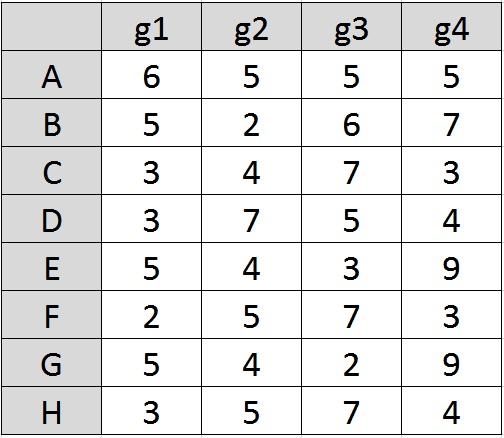
\includegraphics[scale=0.3]{img/AD-Jugement.jpg}
\end{center}
\end{figure}

Nous avons décidé dans notre étude de mener deux expériences. La première sera l'étude des différents projets sans aucune pondération des critères analysés. La seconde proposera une étude basée sur la seconde partie de ce projet, la programmation linéaire multicritère, afin d'accorder une pondération plus importantes aux critères qui auront été jugés plus importants. Après une analyse de ces deux expériences, nous en déduirons la meilleure solution répondant à la demande du client.

\section{Étude 1 : Analyse sans pondération des critères}

\subsection{Simplification de la matrice de jugement}

La première étape de cette analyse réside dans la simplification du tableau de la matrice de jugement. En effet, certains projets sont simplement moins bons que d'autres et il n'est pas intéressant de les inclure dans l'analyse à moins de vouloir polluer les résulats et le graphe résultant.

Dans notre cas, nous remarquons que le projet \textbf{E} domine le projet \textbf{G} en tous critères. Il n'est dont pas primordial de garder dans l'analyse le projet \textbf{G}. De la même façon, nous remarquons que le projet \textbf{H} domine le projet \textbf{F} en tous critères, donc nous pouvons également exclure le projet \textbf{F} de l'analyse.


\subsection{Calcul de la matrice de concordance}

La seconde étape de l'algorithme consiste à réaliser une matrice, nommée matrice de concordance. Cette matrice permet de donner une valeur aux différentes paires de propositions de gestion d'atelier. Nous considérons qu'une paire de propositions est constituée d'un premier projet se situant dans la ligne de la matrice et que le second projet est situé dans la colonne de la matrice. De cette façon, il est possible d'analyser tous les projets les uns par rapport aux autres et de leur attribuer un poids plus ou moins grand en fonction de la supériorité du premier projet par rapport au second. Cette supériorité est déduite en fonction de l'analyse de chaque critère, ceci étant explicité plus loin à l'aide de la formule mathématique associée. 

Après avoir supprimmé les deux projets précédents, nous obtenons donc une matrice de taille 6 x 6 à analyser avec les projets \textbf{A}, \textbf{B}, \textbf{C}, \textbf{D}, \textbf{E} et \textbf{H}. La formule qui nous permet de remplir la matrice de concordance est la suivante :

\[
  C(A_i, A_j) = \frac{\sum\limits_{k \in P^+ \cup P^=}{p_k}}{\sum\limits_{I \in P}{p_I}}
\]

Nous considérons que les lignes de la matrice représentent le projet i et que les colonnes de la matrice représentent le projet j.

Pour faire simple, cette formule consiste, pour chaque paire de projets analysés, à compter combien de fois le projet i est meilleur ou équivalent au projet j. Ce chiffre est divisé par la somme de tous les critères sur lesquels ont été jugés les propositions. Sachant qu'il existe 4 critères, nous diviserons donc tous les résultats par 4.


Après calculs nous obtenons donc la matrice suivante :

\begin{figure}[h]
\begin{center}
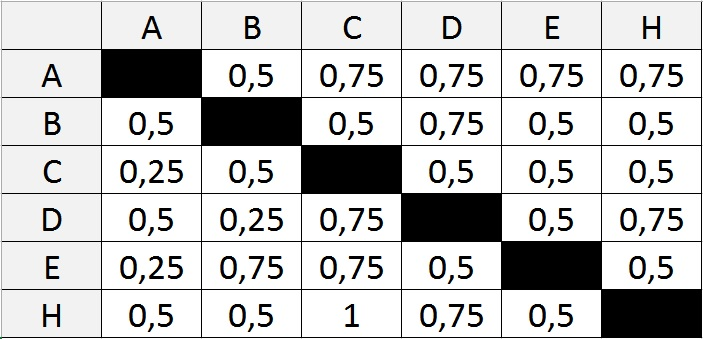
\includegraphics[scale=0.3]{img/AD_Concordance_neutre.jpg}
\end{center}
\end{figure}

\subsection{Calcul de la matrice de discordance}

La troisième étape de l'algorithme consiste à réaliser une autre matrice, nommée matrice de discordance. Cette matrice permet également de donner une valeur aux différentes paires de propositions de gestion d'atelier. De la même façon qu'avec la matrice de concordance, nous considérons qu'une paire de propositions est constituée d'un premier projet se situant dans la ligne de la matrice et que le second projet est situé dans la colonne de la matrice. La valeur qui sera attribuée à chaque paire de propositions correspondra à un écart entre deux critères, écart calculé lorsque le premier projet est moins bon le second projet dans un des critères analysés. Une explication plus en détail est fournie plus loin à l'aide de la formule mathématique associée.

Nous réalisons la matrice de discordance de la même façon que la matrice de concordance à ceci près que les coefficients ne sont pas calculés de la même façon. Nous obtenons une matrice équivalente, de taille 6 x 6 avec les projets \textbf{A}, \textbf{B}, \textbf{C}, \textbf{D}, \textbf{E} et \textbf{H}. La formule qui va nous permettre de remplir cette matrice est la suivante :

\[
  D(A_i, A_j) = \frac{max_{k \in P^-}(e_{jk} - e_{ik})}{echmax}
\]

Nous considérons toujours que les lignes de la matrice représentent le projet i et que les colonnes de la matrice représentent le projet j.

Pour faire simple, cette formule demande, pour chaque critère de chaque paire de projets, de calculer l'écart présent entre le critère du projet i et le critère du projet j lorsque le projet i se révèle moins bon que le projet j au niveau de ce critère. On soustrait donc la valeur du critère du projet j à la valeur du critère du projet i pour chaque critère qui présente ce cas. Il faut ensuite prendre l'écart maximum qui aura été trouvé après l'analyse de chacun des critères. Ce chiffre est ensuite divisé par l'échelle maximum, c'est-à-dire l'écart maximum qui a été utilisé pour la notation des projets dans chacun des critères. Dans notre cas, la note minimale est de 0 et la note maximale est de 10. L'écart sera donc de 10 et nous diviserons donc le résultat pour 10. 

Après calculs nous obtenons donc la matrice suivante :

\begin{figure}[h]
\begin{center}
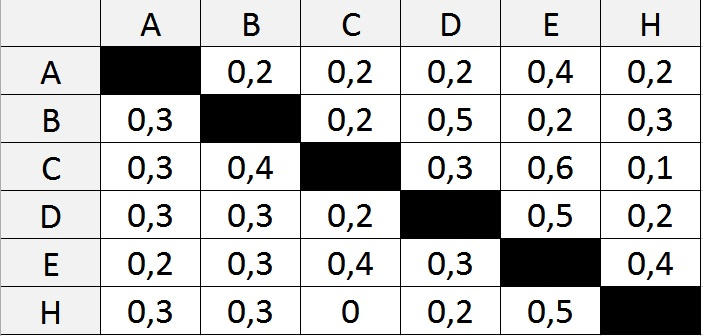
\includegraphics[scale=0.3]{img/AD-Discordance.jpg}
\end{center}
\end{figure}

\subsection{Graphe de surclassement}

Le graphe de surclassement permet d'avoir une vue globale sur les projets et de déterminer quel est le meilleur entre tous. Les points de ce graphe représentent les propositions analysées et les arcs représentent quant à eux le surclassement, c'est-à-dire le fait qu'une proposition \textbf{i} soit supérieure à une proposition \textbf{j} : $ i \longrightarrow j $.

Pour réaliser ce graphe, nous utilisons les matrices de concordance et de discordance ainsi que deux seuils : le seuil de concordance et le seuil de discordance que nous allons définir.

Le seuil de concordance représente le minimum requis en concordance, c'est-à-dire qu'entre deux projets, pour pouvoir dire qu'un projet surclasse effectivement l'autre, il faudra que son indice de concordance soit supérieur ou égal au seuil de concordance. Nous pouvons donc choisir un seuil plus ou moins sévère en fonction des attentes du client. Plus le seuil est élevé, plus le seuil sera sévère et plus la note dans un critère devra être bonne pour que le surclassement soit réprésenté dans le graphe. Nous remarquons également que le seuil doit être compris entre 0,5 et 1 pour avoir un seuil de concordance logique et réaliste. 

Dans notre cas, nous sommes partis d'un seuil de concordance très sévère puis nous avons baissé le degré de sévérité afin d'obtenir un graphe de surclassement avec un nombre d'informations suffisant pour déterminer quel projet est le meilleur.

Cependant, ce seuil de concordance ne doit pas être utilisé seul. Nous devons également utiliser le seuil de discordance qui représente le maximum toléré en discordance. Ce seuil va nous permettre de dessiner ou non sur le graphe un arc en fonction de l'écart qui existe dans le plus mauvais de ses critères. Plus nous prendrons un seuil sévère, plus l'écart devra être serré pour pouvoir effectivement dire qu'un projet surclasse un autre projet. Si le seuil est plutôt indulgent, l'écart pourra être large.

Dans notre cas, nous sommes partis d'un seuil de discordance indulgent puis nous avons baissé le degré de sévérité. 

Voici quatre graphes de surclassement possédant des seuils de concordance et de discordance différents :

\begin{figure}[H]
\begin{center}
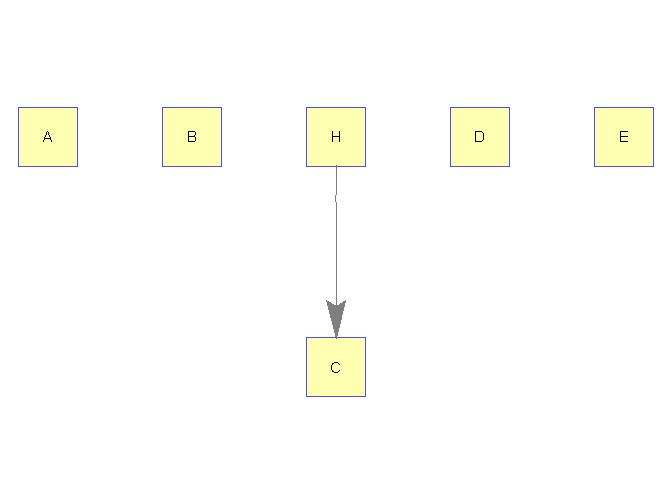
\includegraphics[scale=0.3]{img/G1-neutre.jpg}
\caption{Analyse sans pondération - Seuil de concordance = $\frac{3,75}{4}$ ; seuil de discordance = $\frac{8}{10}$}
\end{center}
\end{figure}

\begin{figure}[H]
\begin{center}
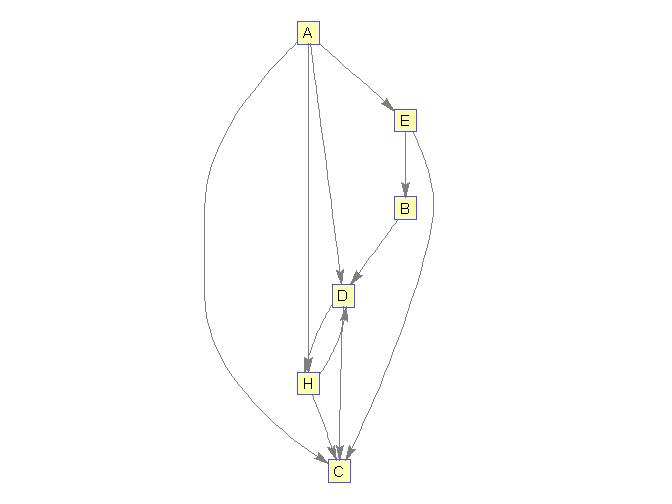
\includegraphics[scale=0.3]{img/G2-neutre.jpg}
\caption{Analyse sans pondération - Seuil de concordance = $\frac{3}{4}$ ; seuil de discordance = $\frac{8}{10}$}
\end{center}
\end{figure}

\begin{figure}[H]
\begin{center}
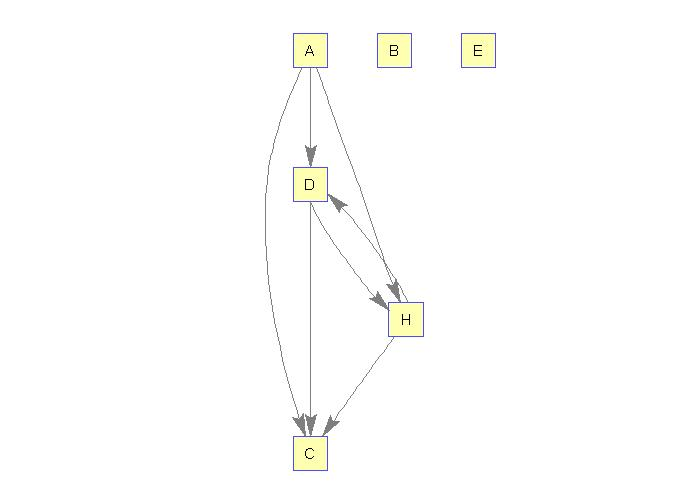
\includegraphics[scale=0.3]{img/G3-neutre.jpg}
\caption{Analyse sans pondération - Seuil de concordance = $\frac{3}{4}$ ; seuil de discordance = $\frac{2}{10}$}
\end{center}
\end{figure}

\begin{figure}[H]
\begin{center}
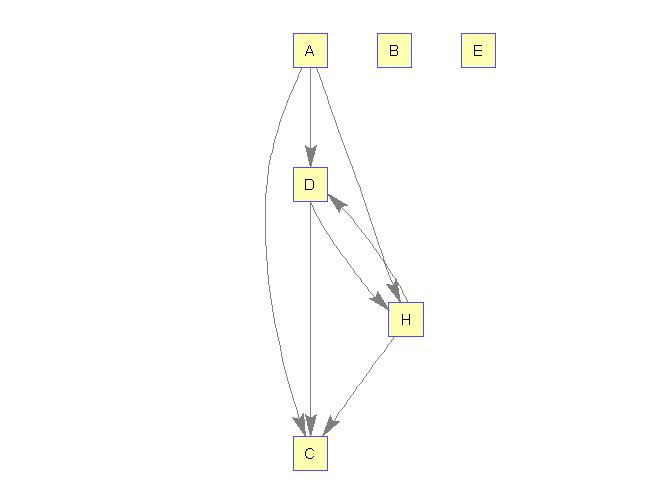
\includegraphics[scale=0.3]{img/G4-neutre.jpg}
\caption{Analyse sans pondération - Seuil de concordance = $\frac{2,5}{4}$ ; seuil de discordance = $\frac{2}{10}$}
\end{center}
\end{figure}

Nous souhaitons être plutôt sévères au niveau du seuil de concordance afin de trouver le meilleur projet, sans l'être trop. En effet, un seuil de concordance trop important n'est pas très représentatif. Les projets risquent de ne pas être assez bons pour être dessinés sur le graphe et ce n'est pas ce qui est recherché. De plus, nous souhaitons que le projet soit plutôt bon dans chacun des critères, d'où l'utilisation d'un seuil de discordance sévère également. Pour la suite de l'étude nous analyserons donc le graphe de surclassement \no3 possédant un seuil de concordance de $\frac{3}{4}$ et un seuil de discordance de $\frac{2}{10}$.

L'analyse du graphe \no3 nous permet de constater que le projet \textbf{A} est le meilleur. En effet, c'est celui qui surclasse tous les autres sans être jamais surclassé. C'est le noyau du graphe et le projet que nous considérerons comme le meilleur pour cette première étude.

\section{Étude 2 : Analyse avec pondération des critères}

Nous avons choisi plusieurs pondérations afin de donner un poids plus important à certains critères. D'après l'étude réalisée dans la deuxième partie de ce compte-rendu, "Programmation linéaire multicritère", nous avons donc décidé de privilégier le critère G1 et de minimiser le poids du critère G4 :

\begin{itemize}
\item Coefficient de pondération de G1 : 4 (le bénéfice)
\item Coefficient de pondération de G2 : 2 (la gestion du stock)
\item Coefficient de pondération de G3 : 2 (l'équilibre commercial)
\item Coefficient de pondération de G4 : 1 (l'utilisation de la machine 4)
\end{itemize}

Nous avons décidé de priviléger le bénéfice au détriment d'une faible utilisation de la machine 4. En effet, en ces temps de crises, il est important que l'entreprise produise un chiffre d'affaire le plus élevé possible. De plus, le fait de diminuer l'utilisation de la machine est un objectif totalement opposé à la génération de bénéfices.

\subsection{Simplification de la matrice de jugement}

De la même façon que dans l'étude \no1, la matrice de jugement est simplifiée en supprimant les projets \textbf{F} et \textbf{G} qui sont dominés respectivement par les projets \textbf{E} et \textbf{H}.

\subsection{Calcul de la matrice de concordance}

La matrice de concordance est calculée de la même façon que dans l'étude \no{1}. Cependant, certaines pondérations ont été ajoutées afin de donner plus de poids aux critères qui ont été jugés plus importants que les autres. Cela modifie donc la matrice de concordance. Lorsque le critère du projet \textbf{i} sera supérieur au même critère du projet \textbf{j}, nous allons donc compter cette valeur en pondérant par le coefficient associé au critère. 

Après calculs nous obtenons donc la matrice suivante :


\begin{figure}[h]
\begin{center}
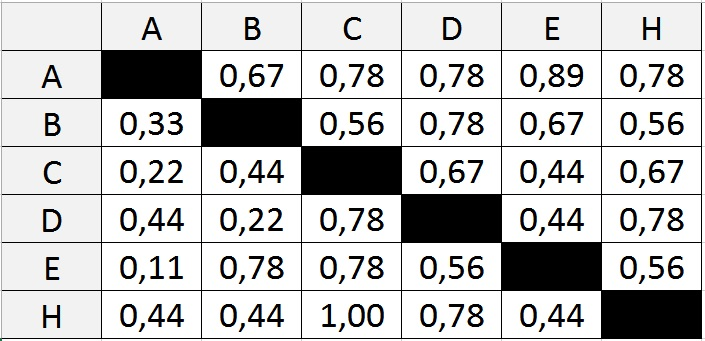
\includegraphics[scale=0.3]{img/AD_Concordance_ponderee.jpg}
\end{center}
\end{figure}

\subsection{Calcul de la matrice de discordance}

En ce qui concerne la matrice de discordance, la pondération associée aux différents critères ne modifie en rien la matrice. Nous obtenons donc la même matrice de discordance calculée lors de la première étude :

\begin{figure}[h]
\begin{center}
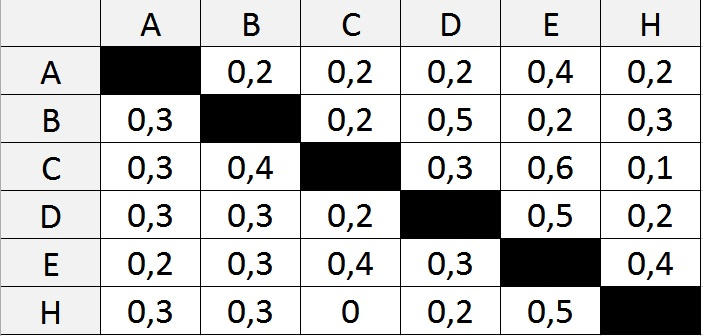
\includegraphics[scale=0.3]{img/AD-Discordance.jpg}
\end{center}
\end{figure}

\subsection{Graphe de surclassement}

De la même façon que pour l'étude \no1, nous sommes partis de de seuils plutôt sévères pour ensuite trouver les seuils les plus représentatifs.

Voici quatre graphes de surclassement possédant des seuils de concordance et de discordance différents :

\begin{figure}[H]
\begin{center}
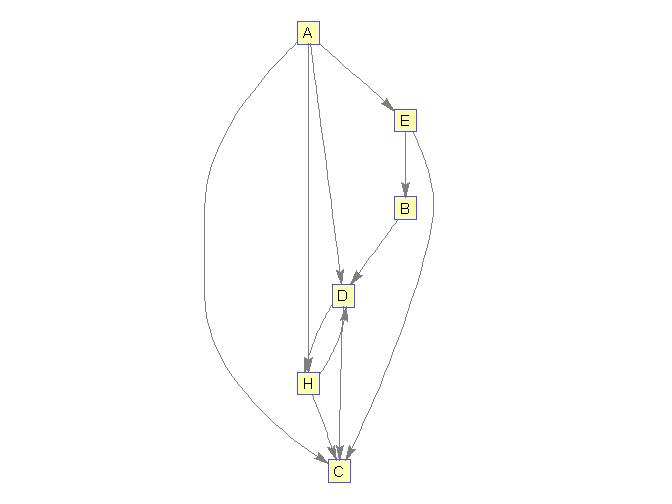
\includegraphics[scale=0.3]{img/G1-pond.jpg}
\caption{Analyse avec pondérations - Seuil de concordance = $\frac{3,75}{4}$ ; seuil de discordance = $\frac{8}{10}$}
\end{center}
\end{figure}

\begin{figure}[H]
\begin{center}
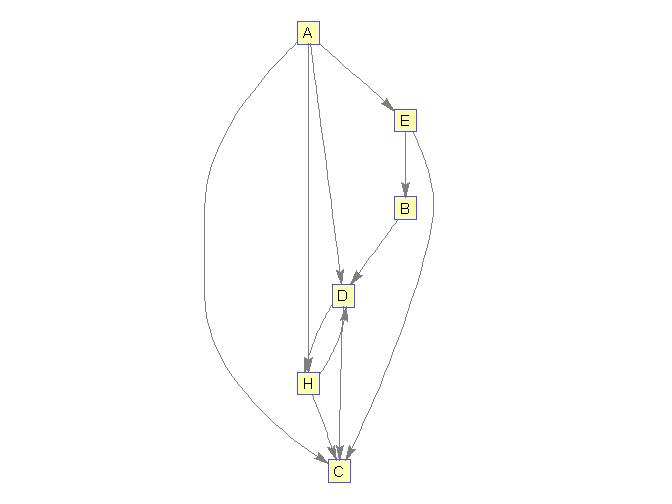
\includegraphics[scale=0.3]{img/G2-pond.jpg}
\caption{Analyse avec pondérations - Seuil de concordance = $\frac{3}{4}$ ; seuil de discordance = $\frac{8}{10}$}
\end{center}
\end{figure}

\begin{figure}[H]
\begin{center}
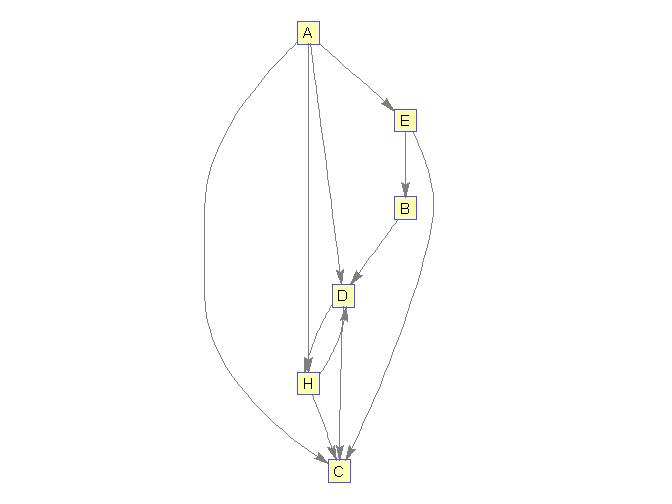
\includegraphics[scale=0.3]{img/G3-pond.jpg}
\caption{Analyse avec pondérations - Seuil de concordance = $\frac{3}{4}$ ; seuil de discordance = $\frac{2}{10}$}
\end{center}
\end{figure}

\begin{figure}[H]
\begin{center}
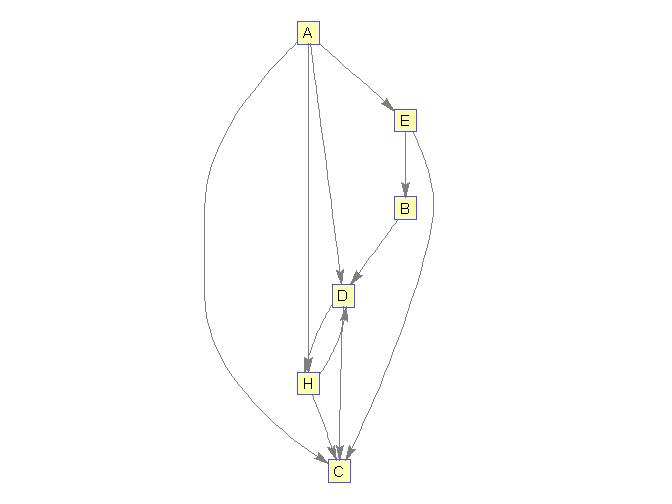
\includegraphics[scale=0.3]{img/G4-pond.jpg}
\caption{Analyse avec pondérations - Seuil de concordance = $\frac{2,5}{4}$ ; seuil de discordance = $\frac{2}{10}$}
\end{center}
\end{figure}

En privilégiant le critère G1 concernant le bénéfice et en minimisant le critère G4 concernant l'utilisation de la machine 4 nous obtenons des graphes assez similaires quels que soient les seuils établis ci-dessus. En effet, le fait d'avoir pondéré les critères permet de converger plus facilement vers le projet respectant le plus les critères importants.

Il s'avère que le noyau de chaque graphe est le projet \textbf{A}. C'est donc le meilleur projet.

Après ces deux études, nous remarquons que le projet \textbf{A} domine tous les autres projets.


%%%%%%%%%%%%%%%%%%%%%%%%%%%%%%%%%%%%%%%%%%%
%%%%%% Partie ANNEXE %%%%%%%%%%%%%%%%%%%%%%
%%%%%%%%%%%%%%%%%%%%%%%%%%%%%%%%%%%%%%%%%%%

\newpage
\part{Annexes}
\appendix

%%%%%%%%%%% Annexe A
\section{Calcul des coefficients pour la modélisation des objectifs du comptable}
\label{annexe}

Le but du comptable est de maximiser le bénéfice global. Pour cela, on doit
calculer le bénéfice à la vente pour chaque produit.

Le bénéfice à la vente correspond au prix de vente du produit fini auquel
on soustrait le coût de fabrication. Le coût de fabrication est composé du
coût en matières premières et coût en utilisation machines.

Pour le coût en utilisation machine, on doit penser à convertir coût horaire
des machines en coût par minute, puisque les temps unitaires d'usinage sont
exprimés en minutes.

Les calculs sont détaillés ci-après :

%Revoir comment écrire les symboles multiplication
On exprime les coûts par minute :
$$ CoutMachine_A = \frac{TempsUsinageMachine_1*CoutHoraireMachine_1 + ...}{60} $$
$$ CoutMachine_A = \frac{8*2+7*2+8*1+2*1+5*2+5*3+5*1}{60} $$
$$ CoutMachine_A = 1,167 $$

On en déduit le bénéfice :
$$ Benefice_A = PrixVente_A - CoutMachine_A - CoutMP_A $$
$$ Benefice_A = 20 - 1,167 - 13 $$
$$ Benefice_A = 5,833 $$

La calcul est analogue pour les autres produits.


%%%%%%%%%%% Annexe B
\newpage
\section{Code source Matlab}
\lstinputlisting{./anal-rapport.m}

\end{document}